Dans ce chapitre nous présentons un langage impératif permettant de modéliser
C. Nous donnons sa syntaxe, une sémantique opérationelle ainsi qu'un
système de types permettant d'obtenir plus de garanties que le système de typse
original de C tel que décrit dans \cite{AnsiC}.

Il permet le polymorphisme sur les types pointeurs, permettant par exemple de
typer :

\begin{mathpar}
⊢ \text{memcpy} : ∀ a . (a^*, a^*, \text{size\_t}) \rightarrow \tVoid
\end{mathpar}

La traduction depuis C sera explicitée dans le chapitre~\ref{cha:implem}.

\section{Syntaxe}

La grammaire suivante définit un langage impératif. On suppose qu'on peut
compiler un programme écrit en C vers ce langage.

Un programme est un triplet $P = (\vec{f}, \vec{x}, b)$ constitué d'un ensemble
de fonctions, d'un ensemble de variables et d'un bloc d'instructions. Ce bloc
sera exécuté au lancement du programme ; il peut par exemple contenir le code
d'initialisation des variables globales et l'appel à la fonction principale.

\gramlr{Programmes}{
\begin{align*}
P \gramisa & (\vec{f}, \vec{v}, b) & \textrm{Fonctions, globales, initialiseur}
\end{align*}
}

\gramlr{Expressions}{
\begin{align*}
e  \gramisa & lv              & \textrm{Left-value}
\\ \gramor  & \textrm{op}~e   & \textrm{Opération unaire}
\\ \gramor  & e~\textrm{op}~e & \textrm{Opération binaire}
\\ \gramor  & cst             & \textrm{Constante}
\\ \gramor  & \& lv           & \textrm{Pointeur sur donnée}
\\ \gramor  & \& f            & \textrm{Pointeur sur fonction}
\end{align*}
}

\gramlr{Opérateurs}{
\begin{align*}
\textrm{op} \gramisa & +,-,\times,/         & \textrm{Arithmétique entière}
\\          \gramor  & +.,-.,\times.,/.     & \textrm{Arithmétique flottante}
\\          \gramor  & =,≠,≤,≥,<,>          & \textrm{Comparaisons}
\\          \gramor  & \&,|,\textasciitilde & \textrm{Opérateurs bit à bit}
\\          \gramor  & \&\&,||,!            & \textrm{Opérateurs logiques}
\\          \gramor  & ⋘, ⋙                 & \textrm{Décalages}
\end{align*}
}

\todo{XOR}

\gramlr{Left-values}{
\begin{align*}
lv \gramisa & var      & \textrm{Variable}
\\ \gramor  & lv.champ & \textrm{Accès à un champ}
\\ \gramor  & lv[e]    & \textrm{Accès à un tableau}
\\ \gramor  & *e       & \textrm{Déréférencement}
\end{align*}
}

\gramlr{Blocs}{
\begin{align*}
b  \gramisa & i ; b & \textrm{Séquence}
\\ \gramor  & ε     & \textrm{Bloc vide}
\end{align*}
}

\gramlr{Instructions}{
\begin{align*}
i  \gramisa & lv \leftarrow e             & \textrm{Affectation}
\\ \gramor  & lv \leftarrow funexp (args) & \textrm{Appel de fonction}
\\ \gramor  & funexp (args)               & \textrm{Appel de procédure}
\\ \gramor  & \npkDecl{nom}{b}            & \textrm{Déclaration}
\\ \gramor  & \npkIf{e}{b}{b}             & \textrm{Alternative}
\\ \gramor  & \npkDoWith{b}{label}        & \textrm{Nommage de bloc}
\\ \gramor  & \npkGoto{label}             & \textrm{Saut en avant}
\\ \gramor  & \npkWhile{b}                & \textrm{Boucle infinie}
\\ \gramor  & \npkReturn{e}               & \textrm{Retour de fonction}
\end{align*}
}

\todo{Fonctions}


\todo{expliquer pourquoi un while expr ne suffit pas}

La différence principale avec C est que les expressions sont sans effets de
bords, donc que leur évaluation peut être faite sans modifier l'environnement.

\section{Sémantique}

Dans cette section, nous définissons une sémantique pour ce langage impératif ;
elle pourra servir à l'implantation d'un interpréteur et à raisonner de manière
formelle sur les programme. Mathématiquement, cela consiste en la définition
d'une relation de transition $\rightarrow$ entre états de l'interpréteur.

Un état est constitué d'une part d'un point de contrôle dans le programme
(section~\ref{sec:cfg}, et d'autre part de l'état $σ$ de la mémoire
(section~\ref{sec:sigma}).

\subsection{Graphe de flot de contrôle}
\label{sec:cfg}

Dans la syntaxe ci-dessus, on peut classifier les instructions en deux familles:
celles qui définissent le flot de contrôle (if, dowith, goto, forever) et celles
qui définissent le flot de données. Une première transformation va transformer
chaque fonction en son graphe de flot de contrôle, défini comme suit :

\begin{itemize}
\item
  les nœuds sont des points de contrôle, qui représentent par exemple
  l'adresse mémoire de l'instruction qui vient d'être exécutée.
\item
  les arêtes sont soit des instructions "de données" (affectation,
  appel de fonction, déclaration), soit des conditions (ie une
  expression).
\end{itemize}

\begin{minipage}{0.5\textwidth}
\begin{Verbatim}[commandchars=\\\{\}]
\PY{k+kt}{int} \PY{n+nf}{gcd}\PY{p}{(}\PY{k+kt}{int} \PY{n}{a}\PY{p}{,} \PY{k+kt}{int} \PY{n}{b}\PY{p}{)}
\PY{p}{\PYZob{}}
    \PY{k}{if} \PY{p}{(}\PY{n}{a} \PY{o}{=}\PY{o}{=} \PY{l+m+mi}{0}\PY{p}{)} \PY{p}{\PYZob{}}
        \PY{k}{return} \PY{n}{b}\PY{p}{;}
    \PY{p}{\PYZcb{}}
    \PY{k}{while} \PY{p}{(}\PY{n}{b} \PY{o}{!}\PY{o}{=} \PY{l+m+mi}{0}\PY{p}{)} \PY{p}{\PYZob{}}
        \PY{k}{if} \PY{p}{(}\PY{n}{a} \PY{o}{\PYZgt{}} \PY{n}{b}\PY{p}{)} \PY{p}{\PYZob{}}
            \PY{n}{a} \PY{o}{=} \PY{n}{a} \PY{o}{-} \PY{n}{b}\PY{p}{;}
        \PY{p}{\PYZcb{}} \PY{k}{else} \PY{p}{\PYZob{}}
            \PY{n}{b} \PY{o}{=} \PY{n}{b} \PY{o}{-} \PY{n}{a}\PY{p}{;}
        \PY{p}{\PYZcb{}}
    \PY{p}{\PYZcb{}}
\PY{p}{\PYZcb{}}
\end{Verbatim}

\end{minipage}
\begin{minipage}{0.5\textwidth}
\begin{Verbatim}[commandchars=\\\{\}]
\PY{n}{int32} \PY{n+nf}{gcd}\PY{p}{(}\PY{n}{int32} \PY{n}{a}\PY{p}{,} \PY{n}{int32} \PY{n}{b}\PY{p}{)} \PY{p}{\PYZob{}}
    \PY{k}{if} \PY{p}{(}\PY{n}{a} \PY{o}{=}\PY{o}{=} \PY{l+m+mi}{0}\PY{p}{)} \PY{p}{\PYZob{}}
      \PY{o}{!}\PY{k}{return} \PY{o}{=} \PY{n}{b\PYZus{}int32}\PY{p}{;}
      \PY{k}{goto} \PY{n}{lbl0}\PY{p}{;}
    \PY{p}{\PYZcb{}}
    \PY{k}{while} \PY{p}{(}\PY{l+m+mi}{1}\PY{p}{)} \PY{p}{\PYZob{}}
        \PY{k}{if} \PY{p}{(}\PY{n}{b} \PY{o}{=}\PY{o}{=} \PY{l+m+mi}{0}\PY{p}{)} \PY{p}{\PYZob{}}
            \PY{k}{goto} \PY{n}{lbl1}\PY{p}{;}
        \PY{p}{\PYZcb{}}
        \PY{k}{if} \PY{p}{(}\PY{n}{a} \PY{o}{\PYZgt{}} \PY{n}{b}\PY{p}{)} \PY{p}{\PYZob{}}
             \PY{n}{a} \PY{o}{=} \PY{n}{a} \PY{o}{-} \PY{n}{b}\PY{p}{;}
        \PY{p}{\PYZcb{}} \PY{k}{else} \PY{p}{\PYZob{}}
             \PY{n}{b} \PY{o}{=} \PY{n}{b} \PY{o}{-} \PY{n}{a}\PY{p}{;}
        \PY{p}{\PYZcb{}}
    \PY{p}{\PYZcb{}}
    \PY{n+nl}{lbl1:}
    \PY{n+nl}{lbl0:}
    \PY{p}{;}
\PY{p}{\PYZcb{}}
\end{Verbatim}

\end{minipage}

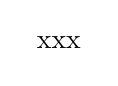
\begin{tikzpicture}
\node{xxx};
\end{tikzpicture}


Intuitivement, on peut "passer" d'un état à un autre soit en passant par une
arête "condition" qui s'évalue à une valeur "vrai", soit en appliquant les
effets de bord d'une arête "instruction".

Dans la suite, on suppose qu'on a à notre disposition un ensemble de jugements :
$\langle l, instr, l' \rangle$ qui signifie qu'on peut passer du point $l$ au
point $l'$ en effectuant l'instruction $instr$.

\subsection{État mémoire}
\label{sec:sigma}

La mémoire interne de l'interpréteur est une correspondance entre l'ensemble des
adresses (infini dénombrable) et l'ensemble des valeurs. Un état mémoire $σ$ est
une fonction partielle de $Addr$ vers $Val$.

Ces valeurs peuvent être de plusieurs formes :

\begin{align*}
v  \gramisa  & n           & \textrm{Entier}
\\ \gramor   & f           & \textrm{Flottant}
\\ \gramor   & \cNil       & \textrm{Pointeur nul}
\\ \gramor   & \&a         & \textrm{Pointeur sur l'adresse $a$}
\\ \gramor   & \&f         & \textrm{Pointeur sur la fonction $f$}
\\ \gramor   & \top        & \textrm{Valeur non initialisée}
\end{align*}

\todo{Pile d'appels}

\subsection{Left values}

La mémoire est organisée en adresses, mais pourtant dans le programme cette
notion n'est pas directement visible. Les accès sont réalisés à travers des
"left values".

\subsection{Jugements}

Les jugements ont les formes suivantes :

\begin{itemize}

\item $σ ⊢ lv ⇒ a$ :
  la left-value lv correspond à l'adresse mémoire a.

\item $σ ⊢ e ⇒ v$ :
  l'expression e s'évalue en v.

\item $(l, σ) \rightarrow (l', σ')$ :
  permet de définir la fonction de transition principale

\end{itemize}

\subsection{Sémantique des left-values}

\begin{mathpar}
\irule{Eval-Lv-Var}{
  (v, a) ∈ σ
}{
  σ ⊢ v ⇒ a
}
\and
\irule{Eval-Lv-Deref}{
  σ ⊢ e ⇒ \&a
}{
  σ ⊢ *e ⇒ a
}
\and
\irule{Eval-Lv-Field}{
  σ ⊢ lv ⇒ a
}{
  σ ⊢ lv.f ⇒ a + f
}
\and
\irule{Eval-Lv-Array}{
  σ ⊢ lv ⇒ a \\
  σ ⊢ e ⇒ n \\
}{
  σ ⊢ lv[e] ⇒ a + n
}
\end{mathpar}

\subsection{Sémantique des expressions}

\begin{mathpar}
\irule{Eval-Cst}{
}{
  σ ⊢ c ⇒ c
}
\and
\irule{Eval-Lv}{
  σ ⊢ lv ⇒ a \\
  (a, v) ∈ σ
}{
  σ ⊢ lv ⇒ v
}
\and
\irule{Eval-Unop}{
  σ ⊢ e ⇒ v
}{
  σ ⊢ \textrm{op}~e ⇒ \widehat{\textrm{op}}~v
}
\and
\irule{Eval-Binop}{
  σ ⊢ e_1 ⇒ v_1 \\
  σ ⊢ e_2 ⇒ v_2
}{
  σ ⊢ e_1~\textrm{op}~e_2 ⇒ v_1 \widehat{\textrm{op}}~v_2
}
\and
\irule{Eval-AddrOf}{
  σ ⊢ lv ⇒ a
}{
  σ ⊢ \&lv ⇒ \&a
}
\and
\irule{Eval-AddrOfFun}{
}{
  σ ⊢ \&f ⇒ \&f
}
\end{mathpar}

\subsection{Sémantique des instructions}

La règle la plus simple concerne l'affectation : on peut affecter une
expressions à une left value si elles ont le même type.

\begin{mathpar}
  \irule{Instr-Assign}{
    \langle l, lv \leftarrow e, l' \rangle \\
    σ ⊢ lv ⇒ a \\
    σ ⊢ e ⇒ v
  }{
    (l, σ) \rightarrow (l', σ [ a ↦ v ])
  }
\end{mathpar}

Déclarer une variable, c'est rendre accessible dans un bloc une variable non
initialisée, qui n'est plus accessible par la suite : Si on suppose qu'on peut
traverser le bloc interne $b$ sous un $σ$ enrichi d'une nouvelle variable $x$,
on peut donc traverser l'instruction $\uparrow x\{b\}$.

\begin{minipage}{0.6\textwidth}
\begin{mathpar}
  \irule{Instr-Decl}{
    \langle l, \uparrow x \{ b \}, l' \rangle \\
    \langle l_b, b, l_b' \rangle \\
    σ' = σ ⊕ \{ x \rightarrow \top \} \\
    (l_b, σ', s) \rightarrow (l_b', σ'')
  }{
    (l, σ) \rightarrow (l', σ'' \backslash x)
  }
\end{mathpar}
\end{minipage}
\begin{minipage}{0.4\textwidth}
\begin{tikzpicture}
  [cfgnode/.style={draw,shape=circle},node distance=2cm]
  \node[cfgnode] (l) {$l$};
  \node[cfgnode,right of=l, node distance=4cm] (lp) {$l'$};
  \node[cfgnode,below of=l, xshift=1cm] (lb) {$l_b$};
  \node[cfgnode,below of=lp, xshift=-1cm] (lbp) {$l_b'$};
  \draw[->] (l)  to node[auto] {$↑x\{b\}$} (lp);
  \draw[->] (lb) to node[auto] {$b$} (lbp);
  \draw[->,dashed] (l) to node[auto] {$⊕ \{ x → \top \}$}(lb);
  \draw[->,dashed,swap] (lbp) to node[auto] {$\backslash x$} (lp);
\end{tikzpicture}

\end{minipage}

\todo{fcall}

TODO pour :

\[
\irule{Instr-Fcall}{
  \langle l, lv \leftarrow fe(\vec{e}), l' \rangle \\
  σ ⊢ fe ⇒ f \\
  σ ⊢ \vec{e} ⇒ \vec{v} \\
  σ' = σ ⊕ \{args(f) = \vec{v}\} ⊕ \{ !ret \rightarrow \top \} \\
  (Entry(f), σ') \rightarrow (Exit(f), σ'') \\
  σ'' ⊢ !ret ⇒ v_{ret} \\
  σ'' ⊢ lv ⇒ a
}{
  (l, σ) \rightarrow (l', σ'' \backslash (args(f) \cup \{!ret\}) ⊕ \{ a \rightarrow v_{ret}\}, ?)
}
\]

\todo{definir $σ ⊢ fe ⇒ f$}

\subsection{Sémantique des conditions}

On utilise un encodage similaire à la déclaration. Tout d'abord, on évalue la
condition dans un contexte $σ$. Si elle s'évalue en un entier non nul, et qu'une
transition à travers le bloc $i_t$ est possible, alors on peut faire passer à
travers le "if".

\begin{minipage}{0.5\textwidth}
\begin{tikzpicture}
  [cfgnode/.style={draw,shape=circle}, node distance=1.5cm]
  \node[cfgnode] (l) {$l$};
  \node[cfgnode,right of=l, node distance=4.5cm] (lp) {$l'$};
  \node[cfgnode,below of=l, xshift=5mm] (lt) {$l_t$};
  \node[cfgnode,below of=lp, xshift=-5mm] (ltp) {$l_t'$};
  \node[cfgnode,above of=l, xshift=5mm] (lf) {$l_f$};
  \node[cfgnode,above of=lp, xshift=-5mm] (lfp) {$l_f'$};
  \draw[->] (l)  to node[auto] {$\npkIf{e}{i_t}{i_f}$} (lp);
  \draw[->] (lt) to node[auto] {$i_t$} (ltp);
  \draw[->] (lf) to node[auto] {$i_f$} (lfp);
  \draw[->,dashed] (l) to node [auto,swap] {$≠0$} (lt);
  \draw[->,dashed] (ltp) to (lp);
  \draw[->,dashed] (l) to node [auto] {$0$} (lf);
  \draw[->,dashed] (lfp) to (lp);
\end{tikzpicture}

\end{minipage}
\begin{minipage}{0.5\textwidth}
\begin{mathpar}
\irule{If-True}{
  \langle l, \iIf{e}{i_t}{i_f}, l' \rangle \\
  σ ⊢ e ⇒ n \\
  n ≠ 0 \\
  \langle l_i, i_t, l_i' \rangle \\
  (l_i, σ) \rightarrow (l_i', σ')
}{
  (l, σ) \rightarrow (l', σ')
}
\and
\irule{If-False}{
  \langle l, \iIf{e}{i_t}{i_f}, l' \rangle \\
  σ ⊢ e ⇒ 0 \\
  \langle l_i, i_f, l_i' \rangle \\
  (l_i, σ) \rightarrow (l_i', σ')
}{
  (l, σ) \rightarrow (l', σ')
}
\end{mathpar}
\end{minipage}

\section{Règles de typage}

Dans cette section, on définit la notion de programme bien typé. L'analyse par
typage permet de vérifier qu'à chaque expression on peut associer un type, et ce
de manière cohérente entre plusieurs utilisations d'une variable.

Un jugement de typage est de la forme $Γ ⊢ e : τ$ et se lit "sous $Γ$, $e$ est
typable en $τ$". Un environnement de typage $Γ$ contient le contexte nécessaire
à l'analyse, c'est à dire le type des fonctions et variables du programme.

Les instructions et blocs, au contraire, n'ont pas de type. On note $Γ ⊢ i$ pour
"sous $Γ$, $i$ est bien typé", c'est à dire que ces sous expressions sont
typables et que les types sont en accord avec le flot de données (par exemple,
pour que l'instruction $lv \leftarrow e$ soit bien typée sous $Γ$, il faut que les types
de $lv$ et de $e$ puissent avoir le même type sous $Γ$).

Les types des valeurs sont :

\begin{align*}
τ   ::=~ & \tInt, \tFloat, \tVoid        & \text{constantes}\\
    |~   &  a                            & \text{variable}\\
    |~   & (τ_1, …, τ_n) \rightarrow τ_r & \text{fonction}\\
    |~   & [τ]                           & \text{tableau}\\
    |~   & τ*                            & \text{pointeur}\\
    |~   & \{ f_1:τ_1
            ,    …
            , f_n:τ_n \}                 & \text{structure}
\end{align*}

\subsection{Schémas de type}

On va associer à chaque variable globale un type. Mais faire de même pourrait
être trop restrictif. En effet, une fonction comme memcpy peut être utilisée
pour copier des tableaux d'entiers, mais aussi de flottants. On va donc associer
un schéma de types à chaque fonction.

\[
  σ ::= ∀ \vec{a} . τ
\]

En associant un schéma de type $σ$ à une fonction $f$, on indique que la
fonction pourra être utilisée avec tout type $τ$ qui est une instanciation de
$σ$.

\subsection{Programme}

Au niveau global, un programme P est bien typé (noté $⊢ P$) s'il existe un
environnement $Γ^0$ permettant de typer ses composantes (les fonctions, les
globales et le bloc d'initialisation).

\[
\irule{Prog}{
  Γ^0 = (\vec{σ}, \vec{τ}) \\
  Γ^0 ⊢ \vec{f} : \vec{σ} \\
  Γ^0 ⊢ \vec{x} : \vec{t} \\
  Γ^0 ⊢ b
}{
  ⊢ (\vec{f}, \vec{x}, b)
}
\]

\subsection{Flot de contrôle}

Les règles suivantes permettent de définir les jugements $Γ ⊢ i$. En résumé, les
instructions sont bien typées si leurs sous-instructions sont bien typées. La
seule règle supplémentaire concerne la condition du $if$ qui doit être typée en
\tInt.

\begin{mathpar}
\irule{Pass}{
}{
  Γ ⊢ ε
}
\and
\irule{Seq}{
  Γ ⊢ s \\
  Γ ⊢ b
}{
  Γ ⊢ s;b
}
\and
\irule{Forever}{
  Γ ⊢ b
}{
  Γ ⊢ forever \{ b \}
}
\and
\irule{If}{
  Γ ⊢ e : \tInt \\
  Γ ⊢ i_t \\
  Γ ⊢ i_f
}{
  Γ ⊢ \iIf{e}{i_t}{i_f}
}
\and
\irule{Goto}{
}{
  Γ ⊢ goto l
}
\and
\irule{DoWith}{
  Γ ⊢ b
}{
  Γ ⊢ \{ b \} l:
}
\end{mathpar}

\subsection{Left values}

On étend la relation de typage aux left values : chaque left value, vue comme
une expression, peut être typée.

\begin{mathpar}
\irule{Lv-Var}{
  (v, τ) ∈ Γ
}{
  Γ ⊢ v : τ
}
\and
\irule{Lv-Field}{
  Γ ⊢ lv : τ_s \\
  (f, τ_f) ∈ τ_s
}{
  Γ ⊢ lv.f : τ_f
}
\and
\irule{Lv-Deref}{
  Γ ⊢ e : τ*
}{
  Γ ⊢ *e : τ
}
\and
\irule{Lv-Array}{
  Γ ⊢ lv : [τ] \\
  Γ ⊢ e : \tInt
}{
  Γ ⊢ lv[e] : τ
}
\end{mathpar}

\subsection{Expressions}

\begin{mathpar}
\irule{Const-Int}{
}{
  Γ ⊢ n : \tInt
}
\and
\irule{Const-Float}{
}{
  Γ ⊢ f : \tFloat
}
\and
\irule{Const-Nil}{
}{
  Γ ⊢ \cNil : τ*
}
\and
\irule{Op-Int}{
  op ∈ \{+,-,\times,/,\&,|,\&\&,||,⋘,⋙\} \\
  Γ ⊢ e_1 : \tInt \\
  Γ ⊢ e_2 : \tInt
}{
  Γ ⊢ e_1 op e_2 : \tInt
}
\and
\irule{Op-Float}{
  op ∈ \{+.,-.,\times.,/.\} \\
  Γ ⊢ e_1 : \tFloat \\
  Γ ⊢ e_2 : \tFloat
}{
  Γ ⊢ e_1 \mathrm{op}~ e_2 : \tFloat
}
\and
\irule{Op-Cmp}{
  op ∈ \{=,≠,≤,≥,<,>\} \\
  Γ ⊢ e_1 : τ \\
  Γ ⊢ e_2 : τ \\
  τ ∈ \{ \tInt, \tFloat \}
}{
  Γ ⊢ e_1  \mathrm{op} e_2 : \tInt
}
\and
\irule{Unop-Minus}{
  τ ∈ \{ \tInt, \tFloat \} \\
  Γ ⊢ e : τ
}{
  Γ ⊢ -e : τ
}
\and
\irule{Unop-Not}{
  op ∈ \{ \tilde, ! \}
  Γ ⊢ e : \tInt
}{
  Γ ⊢ op e : \tInt
}
\and
\irule{AddrOf}{
  Γ ⊢ lv : τ
}{
  Γ ⊢ \&lv : τ*
}
\and
\irule{AddrOfFun}{
  Γ ⊢ f : σ \\
  τ ≤ σ
}{
  Γ ⊢ \&lv : τ
}
\end{mathpar}

\subsection{Fonctions}

Pour typer une fonction, on commence par ajouter ses paramètres dans
l'environnement de typage, et on type la définition de la fonction. Le type
résultant est généralisé.

\[
\irule{Fun}{
  Γ' = Γ ⊕ \{ args(f) = \vec{τ} \} \\
  Γ' ⊢ body(f) \\
  Γ' ⊢ !ret : τ_r
}{
  Γ ⊢ f : Gen(\vec{τ} \rightarrow τ_r, Γ)
}
\]

\subsection{Instructions}

\begin{mathpar}
\irule{Decl}{
  Γ ⊕ \{x : τ\} ⊢ b
}{
  Γ ⊢ \uparrow x \{b\}
}
\and
\irule{Assign}{
  Γ ⊢ lv : τ \\
  Γ ⊢ e  : τ
}{
  Γ ⊢ lv \leftarrow e
}
\and
\irule{Fcall}{
  Γ ⊢ lv : τ_{ret} \\
  Γ ⊢ fe : σ \\
  Γ ⊢ \vec{e} : \vec{τ} \\
  (\vec{τ} \rightarrow τ_r) ≤ σ
}{
  Γ ⊢ lv \leftarrow fe(\vec{e})
}
\end{mathpar}

\section{Limitations}
\subsection{Programmes non typables}
\subsection{Incohérences}
